%! Author = guney
%! Date = 03-Aug-25

% Document
\section{Modeling Methodology}\label{sec:modeling-methodology}
\subsection{Overview}\label{subsec:overview}
    MacroSim bases its discovery process on top of a simple $AR(n)$ process where $n$ defines the number of lags for the target variable.
    The constant $c$ and error term $\epsilon$ are assumed 0 and inclusion of noise and linear offest is offloaded to the discovery engine.
    \\

    To aid discovery, supplementary variables are selected from the feature space through the use of \href{https://en.wikipedia.org/wiki/Granger_causality}{ Granger Causality Tests (GCT)} and \href{https://en.wikipedia.org/wiki/Augmented_Dickey%E2%80%93Fuller_test}{Augmented Dickey–Fuller Tests (ADF)}.
    This creates a set of variables that are either direct lags of the target, or are both stationary and have a Granger causal relationship with the target.
    \\

    A symbolic regressor (SR) is responsible for patching these variables in a meaningful way while fitting the AR weights simultaneously.
    Denoting the target as $y$ and the supplementary features as $X_i$, the ultimate resulting expression follows the form $f(AR_y(n), X_1, \dots, X_i)$.
    This process applied to all variables in the feature space to produce a complete and self-sustaining simulation model.

\subsection{Data Preparation}\label{subsec:data-preparation}
\subsubsection{Collection and Formatting}
    MacroSim requires a dataset of time series with matching dates and frequencies.
    There are methods implemented to get, re-index, impute, and format data directly through methods supplied in the library\footnote[1]{See \autoref{subsec:module-structure}\label{fn1}}.
    The data is expected to be in a \texttt{pandas.DataFrame} with a \texttt{DatetimeIndex} and is expected to be entirely numeric.
    There are no expected encoding specifications for categorical variables, but symbolic regression may yield better results with \href{https://en.wikipedia.org/wiki/One-hot}{One-hot Encoding} due to the possibility of having individual coefficients for each category.

\subsubsection{Splitting}
    The target variable is passed to the \texttt{AutoReg} class as a string.
    The processing steps of splitting the features, and creating train/test splits are handled internally.
    \texttt{AutoReg} contains methods to batch and shuffle the data to prevent overfitting due to ordered data and utilize an ensemble learning technique for further robustness.

\subsubsection{Inter-Process Data Transmission}
    Due to the limitations with the dependencies of \texttt{MacroSim}, creating thread pools with shared memory is not possible.
    To allow true parallelism, \texttt{\_batch\_fit} and \texttt{AutoReg} communicate by stripping the non-serializable portions of the model and its output.
    This effectively destroys all but the fitted equation as a string and some limited metadata.
    The equations are converted to \texttt{sympy.Expr} objects and serialized through \texttt{pickle}.
    Upon loading the equations, the metadata is used to reconstruct the model as a native python callable through \texttt{sympy.lambdify}.
    \\

    \texttt{\_Predictor} and \texttt{\_BatchedPredictor} classes wrap these callables and define the standard methods expected to exist in a fitted model.
    (mainly \texttt{predict} and some scoring functions)

\subsection{Target Lag Selection}\label{subsec:target-lag-selection}
    By default, lags of the target feature are configured to cover a 2-year period of observations.
    (two complete cycles of seasonality in many economic contexts)
    This is adjustable through the \texttt{AutoReg.n\_lags}\footref{fn1} attribute, which will be automatically populated with the default lag count using the formula $n_{lags}=2s$ where $s$ denotes the inferred yearly observation frequency.
    \\

    Importantly, lag generation causes data to be shifted, which results in a loss of the first $n_{lags}$ observations.
    Alongside other processes such as training and testing set generation, this can lead to a sizable decrease in usable observations.

\subsection{Feature Selection}\label{subsec:feature-selection}
\subsubsection{Granger Causality}\label{subsubsec:granger-causality}
    By definition, Granger causality tests the predictive power of a variable's past values on the current value of the target.
    Informally, the test structure can be denoted as follows:
    \begin{gather*}
        H_0: X_{t-i} \cancel{\underset{\text{granger-causes}}{\to}} y\\
        H_1: X_{t-i} \underset{\text{granger-causes}}{\to} y\\
    \end{gather*}

    GCTs can take bivariate and multivariate forms; however, MacroSim strictly uses the bivariate form.
    Multivariate GCTs deem if a pair of variables Granger cause the target, but present no further information on the significance of the individual variables.
    This structure necessitates making assumptions to assess and score each variable.
    \\

    Multiple test statistics can be used to determine the significance of the relationship, such as the F-statistic, Chi-squared statistic, and the likelihood ratio.
    MacroSim adopts the F-statistic and performs local causality tests over slices of the data.
    The slices are sized to cover an 8-year period, and the \texttt{max\_lag} parameter is dynamically set through the formula:
    \begin{equation*}
        max\_lag = \rnd*{\frac{N_{obs}}{20\cdot freq}\cdot \ln (N_{obs})}
    \end{equation*}

    This formula provides an almost linear increase in lag size for larger datasets, while smaller datasets receive more conservative lag sizes.

    \begin{figure}[h]
      \centering
      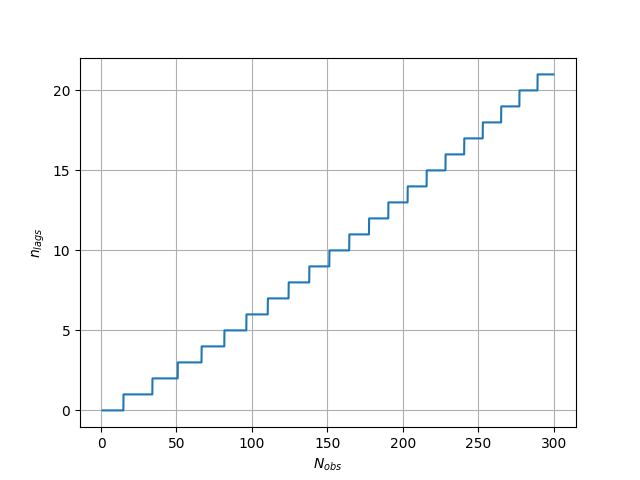
\includegraphics[width=\linewidth]{./assets/Figure_1}
      \caption{Function output for quarterly frequency up to 300 observations.}
      \label{fig:quarterly-output}
    \end{figure}

\subsubsection{Stationarity Tests}\label{subsubsec:stationarity-tests}
    Stationary series are more likely to be robust and reliable features due to their consistent statistical properties over time.
    Features with non-stationary behavior can exhibit different trends at test time, compared to the training time.
    Although shuffling and batching can combat this by incorporating a random sample of observations into training, MacroSim offers the option to filter out non-stationary features.
    \\

    MacroSim takes a simple approach to defining and executing stationarity tests.
    An ADF test is performed on each feature, for lags up to $ \texttt{n\_lags} = \cei*{\sqrt{N_{obs}}} $.
    Macroeconomic variables tend to have trends that evolve over time, directly contradicting the assumptions of stationarity.
    Therefore, the ADF tests are computed for $\alpha = 0.2$.
    Despite the high significance level, and the correspondingly large critical region, it is very possible that the majority of the features will be non-stationary.
    MacroSim implements a warning to inform users of this and encourages testing/caution before asserting stationarity in the feature space.

\subsection{Equation Discovery}\label{subsec:equation-discovery}
\subsubsection{Equation Components}\label{subsubsec:equation-components}
    Although the equation discovery is ultimately handled through SR, it is important to know and navigate the parameters and components of the search space to limit the scope of the search.
    SR is infamously prone to overfitting due to its evolutionary search algorithms.
    It has the ability to add, remove, and modify terms or constants to precisely fit the curve which is very powerful compared to more static regression methods.
    The models are not meant to run at default parameters in most cases, and incorporating domain knowledge into the configuration is essential to avoid overfitting and ensure the model's robustness.
    \\

    MacroSim uses \texttt{PySRRegressor} of the \texttt{pysr} library to perform symbolic regression.
    All \texttt{PySRRegressor} parameters are directly accessible to users and some defaults\footnote[2]{No parameters that change the model weights, or evolution behavior are adjusted. Changes were made to parameters concerning complexity constrataints, allowed operations, model size, and iteration limits.} are modified to better suit the macroeconomic context.
    The model receives a \texttt{TemplateExpressionSpec} as a parameter that defines the structure of function inputs, and can restrict the shapes the function can take.
    \\

    The model has access to $\sin(x)$, $\cos(x)$, $\tan(x)$, $e^x$, $\sqrt{x}$, and $\ln(x)$ as unary operators, while basic arithmetic and exponentiation are available as binary operators.
    The maximum allowed complexity of the variable $x$ can be constrained for each of these operators individually.

\subsubsection{Evolutionary Search}\label{subsubsec:evolutionary-search}
    The search algorithm implemented in \texttt{pysr} is simple in its fundamentals.
    This allows users to have a general idea on where the search will start and how its first few evolutionary steps are likely to progress.
    For illustration, in all configurations, the search starts with the function $f(X) = X$ where $X$ is any of the available features.
    In most model configurations, early evolutions lead toward a simple linear form $f(X) = aX + b$ and the model continues to build more complex expressions.
    \\

    For MacroSim's purposes, the initial expression being $f(X) = X$ is very important as it guarantees that the \texttt{PySRRegressor} will take at least \texttt{n\_iterations} steps on this simple form, before adding an evolutionary component.
    Having a template expression containing the AR process results in the initial expression $f(AR(X)) = AR(X)$ allows the model to exclusively focus on the weights during these initial steps and the rest of the search essentially serves the purpose of a secondary model fitted to the residuals of the AR process.

\subsection{Recursive Simulation}\label{subsec:recursive-simulation}
    \dots



